En esta seccion vamos a realizar una conclusi\'on general de los distintos algoritmos. En base a la performance de los mismos y las distancias con respecto a la soluci\'on Exacta.

Primero planteamos un experimento en el cual corrimos para instancias aleatoreas, nuevamente con las tres densidades utilizadas a lo largo de todo el Trabajo Pr\'actico(15\%, 50\% y 100\%), todos los algoritmos (Exacto con podas, Heuristica Golosa, Heuristica de Busqueda Local y Heuristica GRASP con 5, 15 y 40 oteracioens respectivamente) unas 50 veces para cada cantidad de nodos entre 5 y 20 (por ser numeros manejables para el algoritmo exacto) para sacar un promedio de cuanto difiere cada Heuristica contra el algoritmo Exacto.\\
Para esto calculamos la peor soluci\'on para cada instancia (que ser\'ia ubicar todos los nodos en una \'unica partici\'on, con lo cual la sumatoria de las aristas intrapartici\'on ser\'a la sumatoria total de las aristas) y generamos una formula que nos representa un valor entre 1 y 0 que tanto diverge la Heuristica en relaci\'on al exacto, pero considerando el valor entre la peor soluci\'on y la soluci\'on ideal.
La formula es: 

\bc
1 - ((solucionHeuristica - solucionExacto)/(peorSolucion - solucionExacto))
\ec

Si la Heuristica tiene el mismo valor que el Exacto esta relaci\'on nos devuelve que es 1. Todo lo contrario si la heuristica devuelve la peor soluci\'on, esta formula nos retorna 0.\\
Con lo cual es un buen indicador para saber cuan buena es la soluci\'on de una de las heuristicas.

\subsection{Divergencia de las Heuristicas}

\subsubsection{2 Particiones}

\begin{figure}[H]
\begin{center}
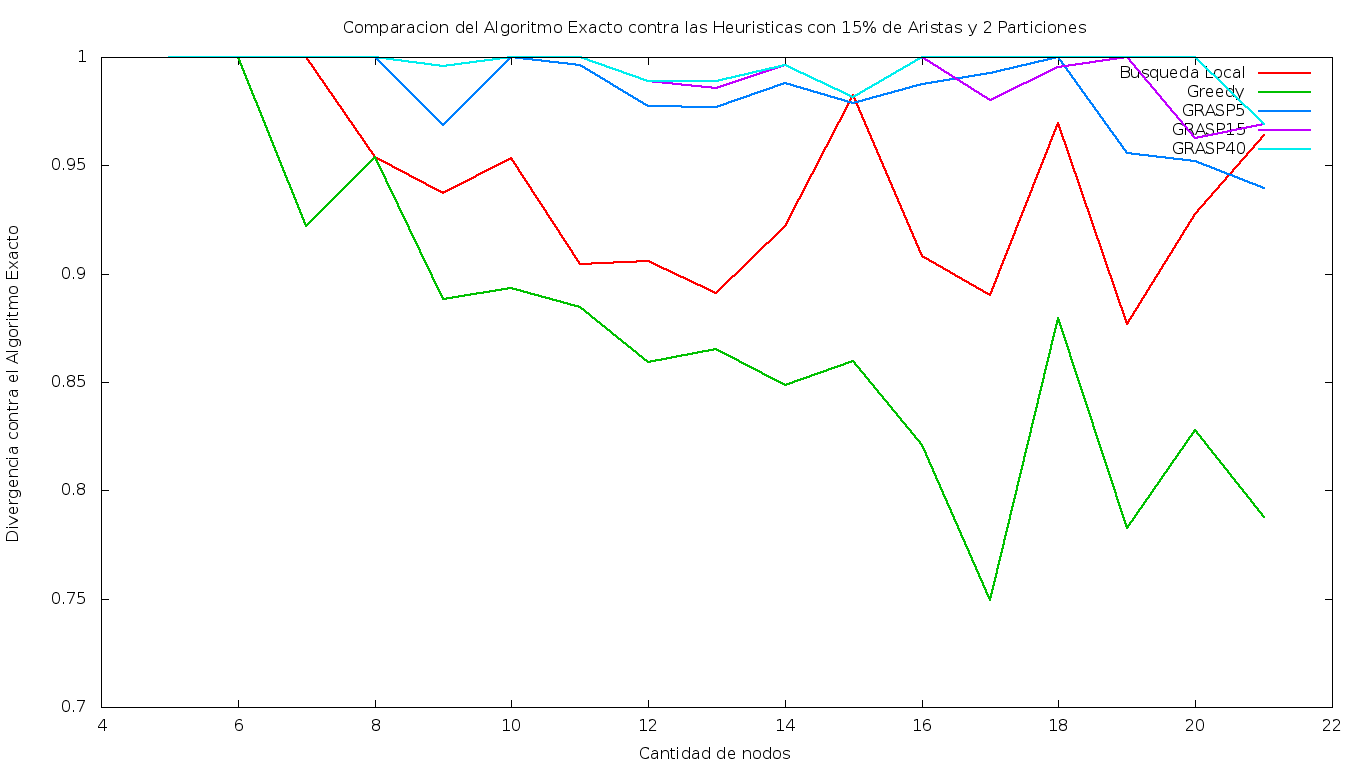
\includegraphics[scale=0.3]{finales/ComparacionesCon2Particiones15Aristas.png}
\caption{Distancias de las Heuristicas para K = 2 y 15\% de aristas}
\end{center}
\end{figure}

\begin{figure}[H]
\begin{center}
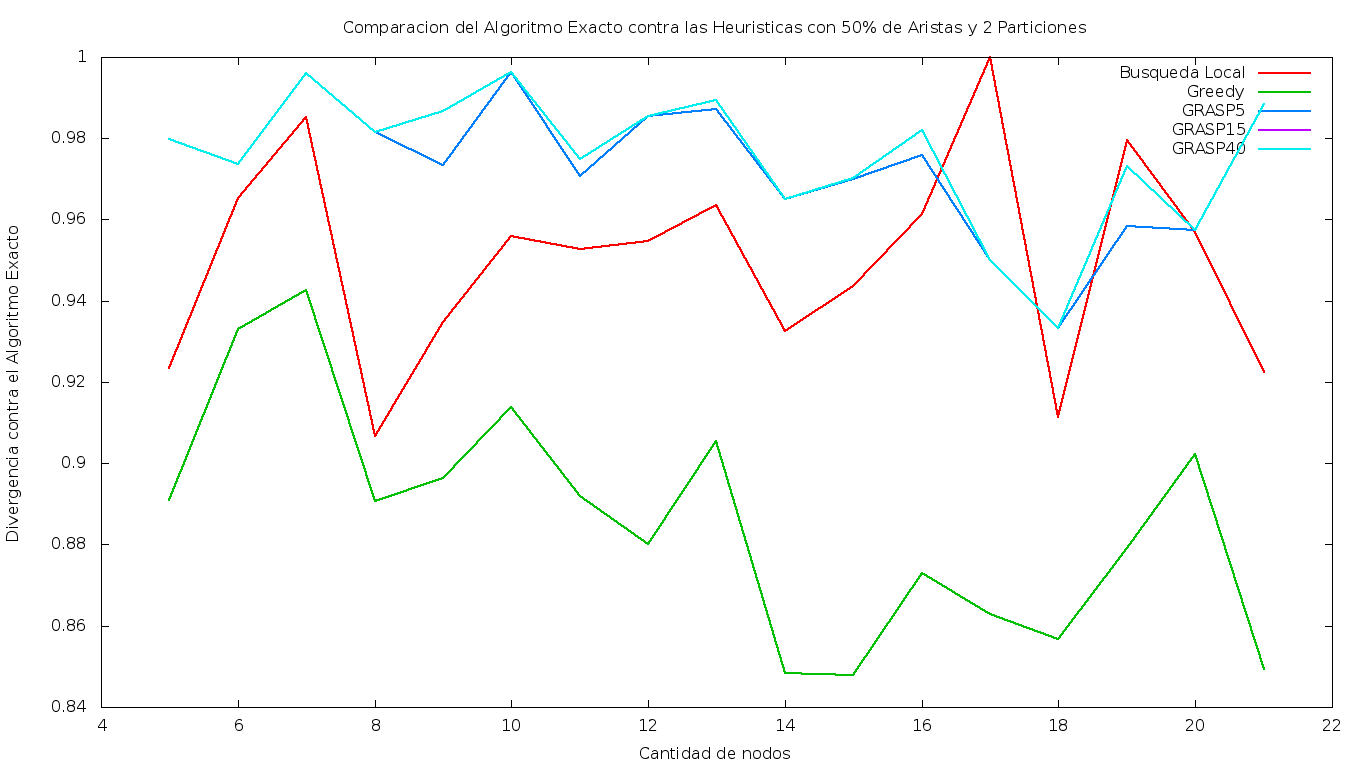
\includegraphics[scale=0.3]{finales/ComparacionesCon2Particiones50Aristas.png}
\caption{Distancias de las Heuristicas para K = 2 y 50\% de aristas}
\end{center}
\end{figure}

\begin{figure}[H]
\begin{center}
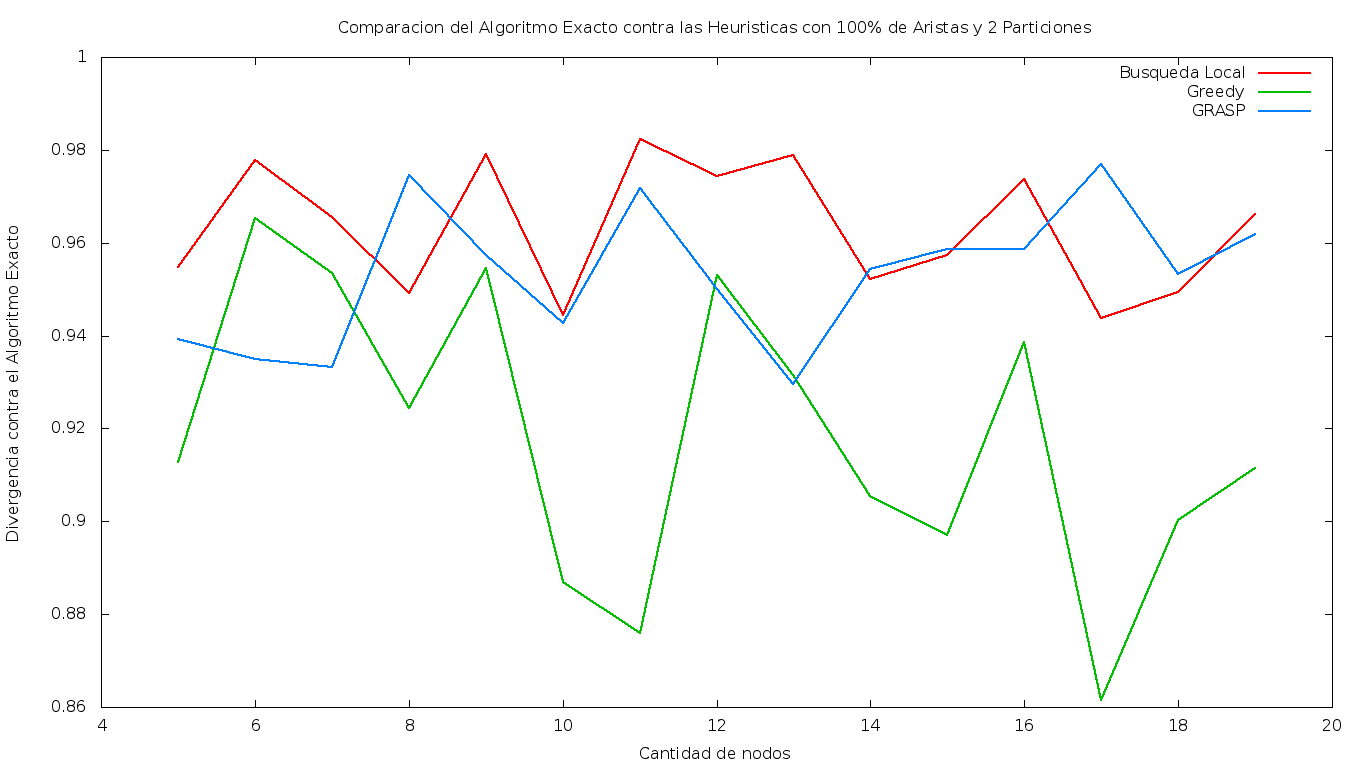
\includegraphics[scale=0.3]{finales/ComparacionesCon2Particiones100Aristas.png}
\caption{Distancias de las Heuristicas para K = 2 y 100\% de aristas}
\end{center}
\end{figure}

\subsubsection{3 Particiones}

\begin{figure}[H]
\begin{center}
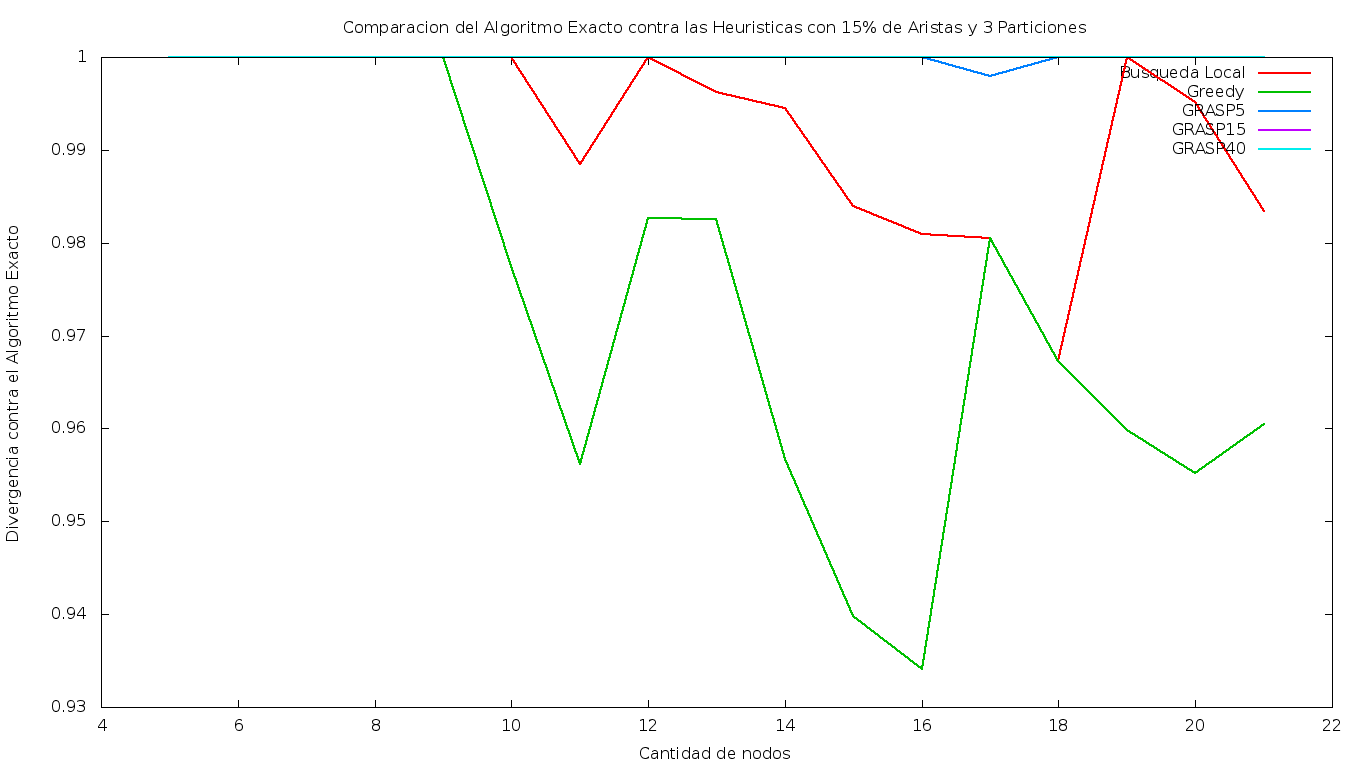
\includegraphics[scale=0.3]{finales/ComparacionesCon3Particiones15Aristas.png}
\caption{Distancias de las Heuristicas para K = 3 y 15\% de aristas}
\end{center}
\end{figure}

\begin{figure}[H]
\begin{center}
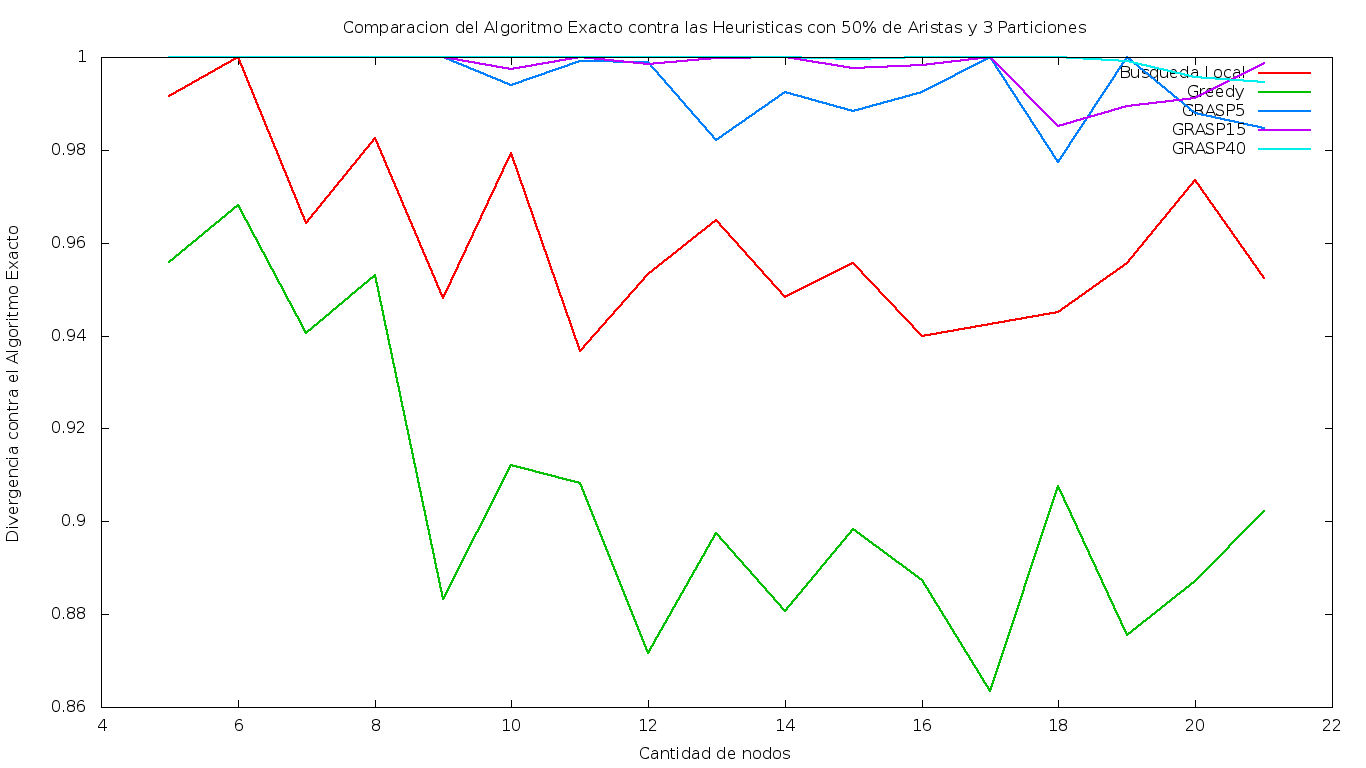
\includegraphics[scale=0.3]{finales/ComparacionesCon3Particiones50Aristas.png}
\caption{Distancias de las Heuristicas para K = 3 y 50\% de aristas}
\end{center}
\end{figure}

\begin{figure}[H]
\begin{center}
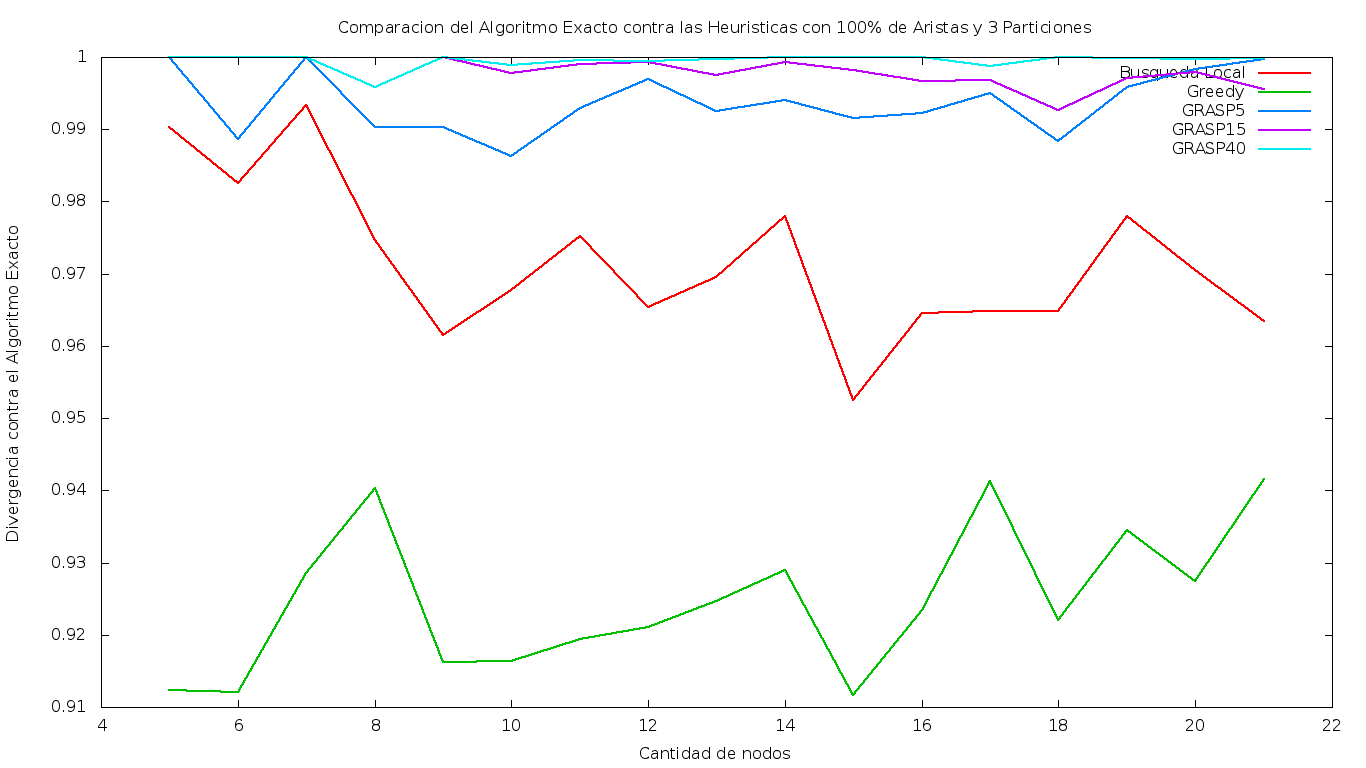
\includegraphics[scale=0.3]{finales/ComparacionesCon3Particiones100Aristas.png}
\caption{Distancias de las Heuristicas para K = 3 y 100\% de aristas}
\end{center}
\end{figure}


\subsubsection{4 Particiones}

\begin{figure}[H]
\begin{center}
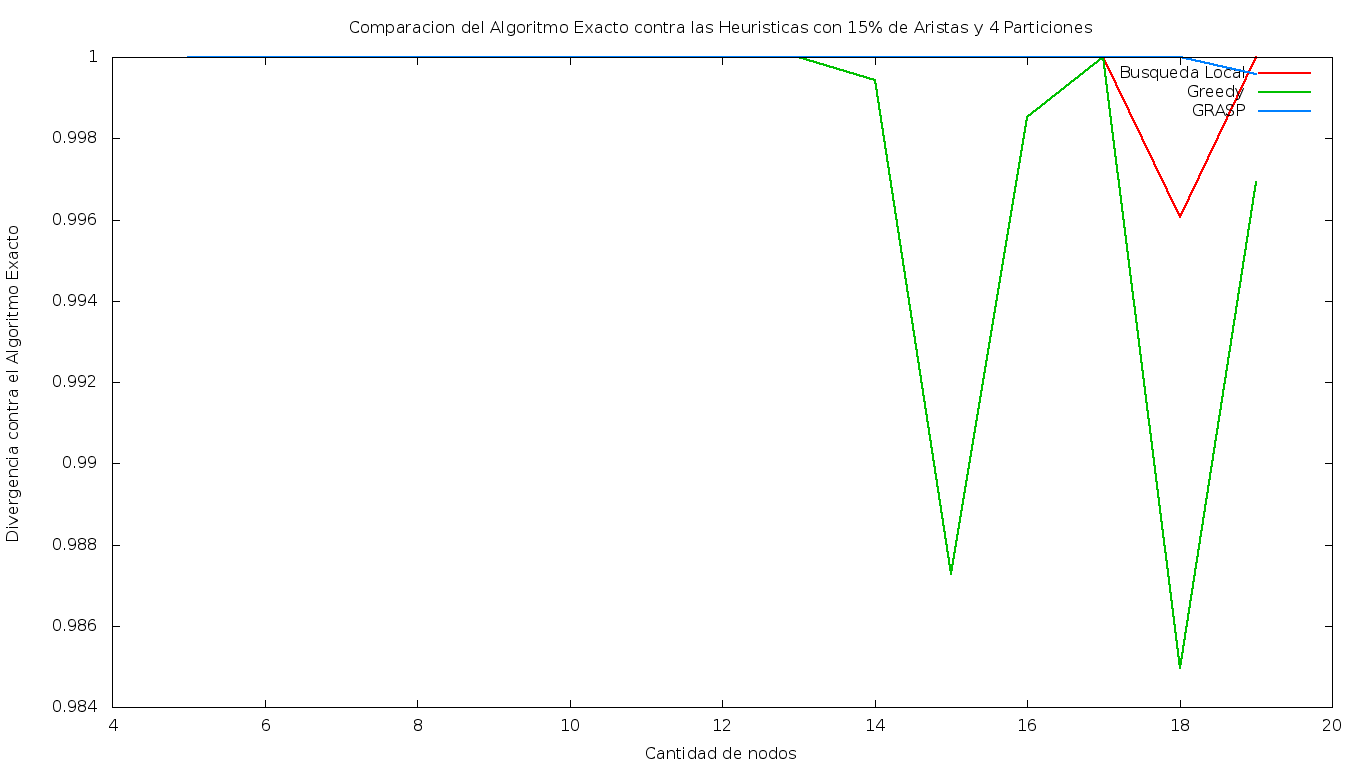
\includegraphics[scale=0.3]{finales/ComparacionesCon4Particiones15Aristas.png}
\caption{Distancias de las Heuristicas para K = 4 y 15\% de aristas}
\end{center}
\end{figure}

\begin{figure}[H]
\begin{center}
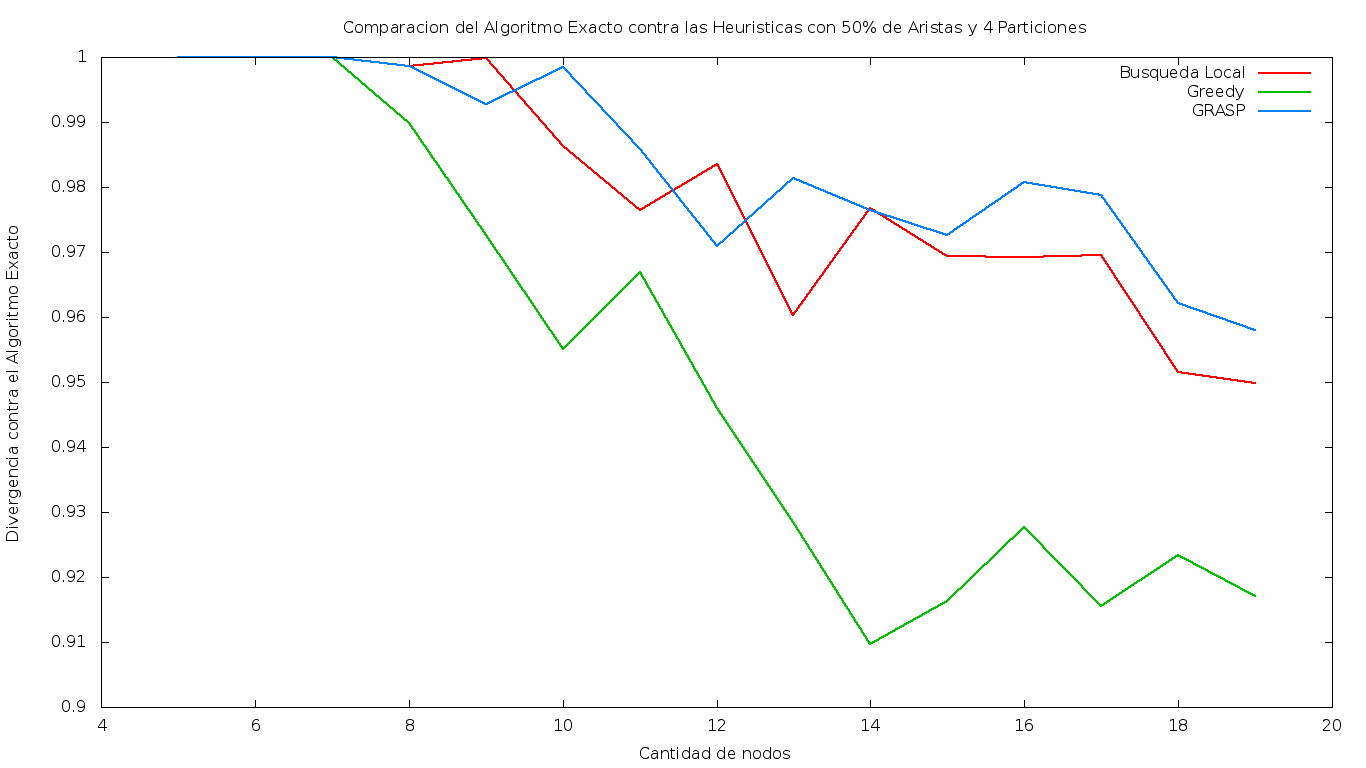
\includegraphics[scale=0.3]{finales/ComparacionesCon4Particiones50Aristas.png}
\caption{Distancias de las Heuristicas para K = 4 y 50\% de aristas}
\end{center}
\end{figure}

\begin{figure}[H]
\begin{center}
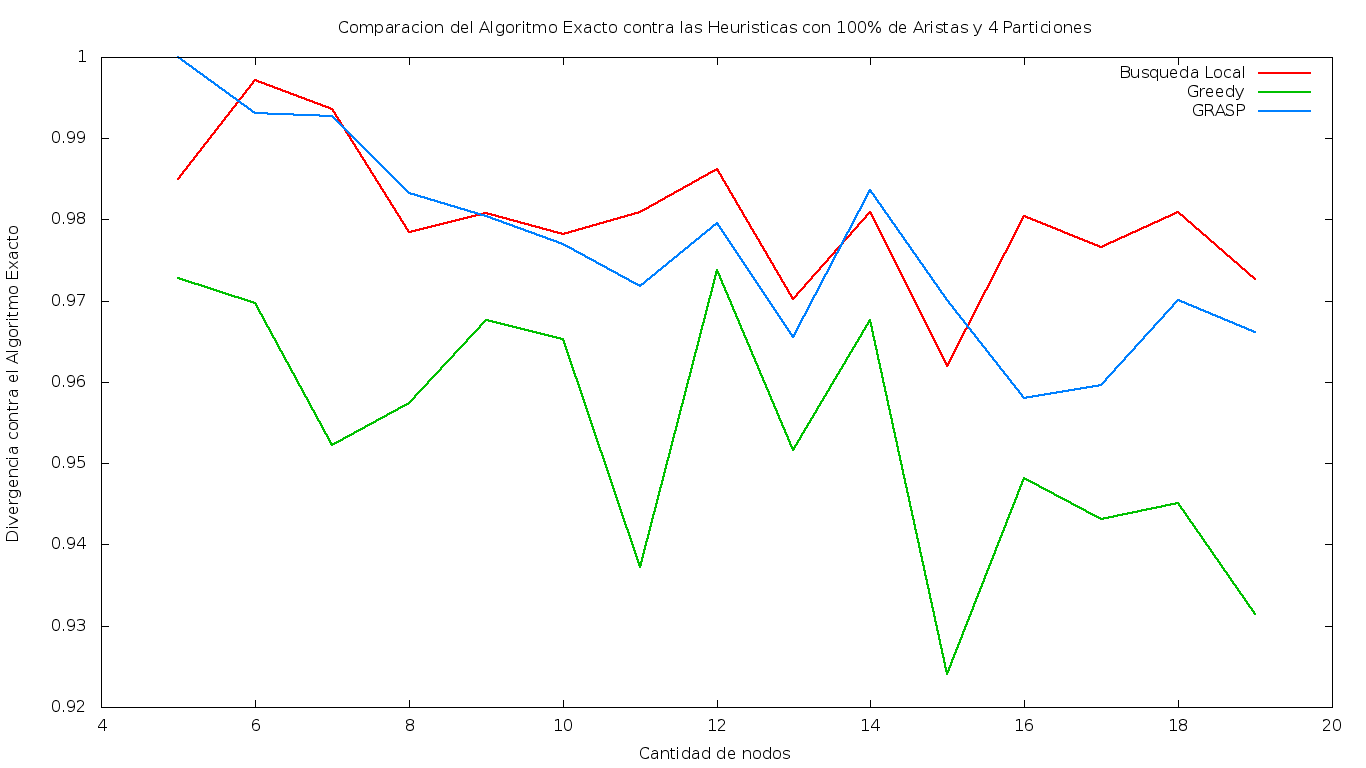
\includegraphics[scale=0.3]{finales/ComparacionesCon4Particiones100Aristas.png}
\caption{Distancias de las Heuristicas para K = 4 y 100\% de aristas}
\end{center}
\end{figure}

\subsubsection{5 Particiones}

\begin{figure}[H]
\begin{center}
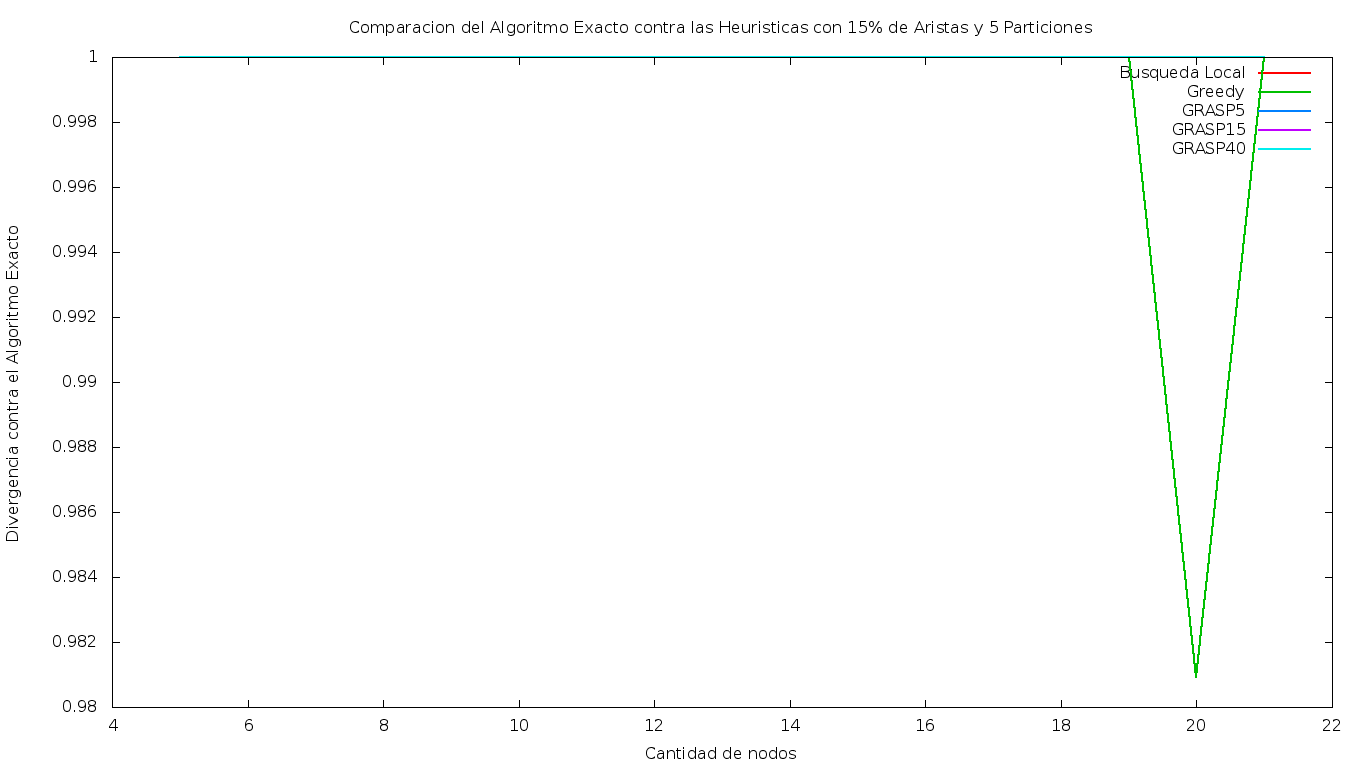
\includegraphics[scale=0.3]{finales/ComparacionesCon5Particiones15Aristas.png}
\caption{Distancias de las Heuristicas para K = 5 y 15\% de aristas}
\end{center}
\end{figure}

\begin{figure}[H]
\begin{center}
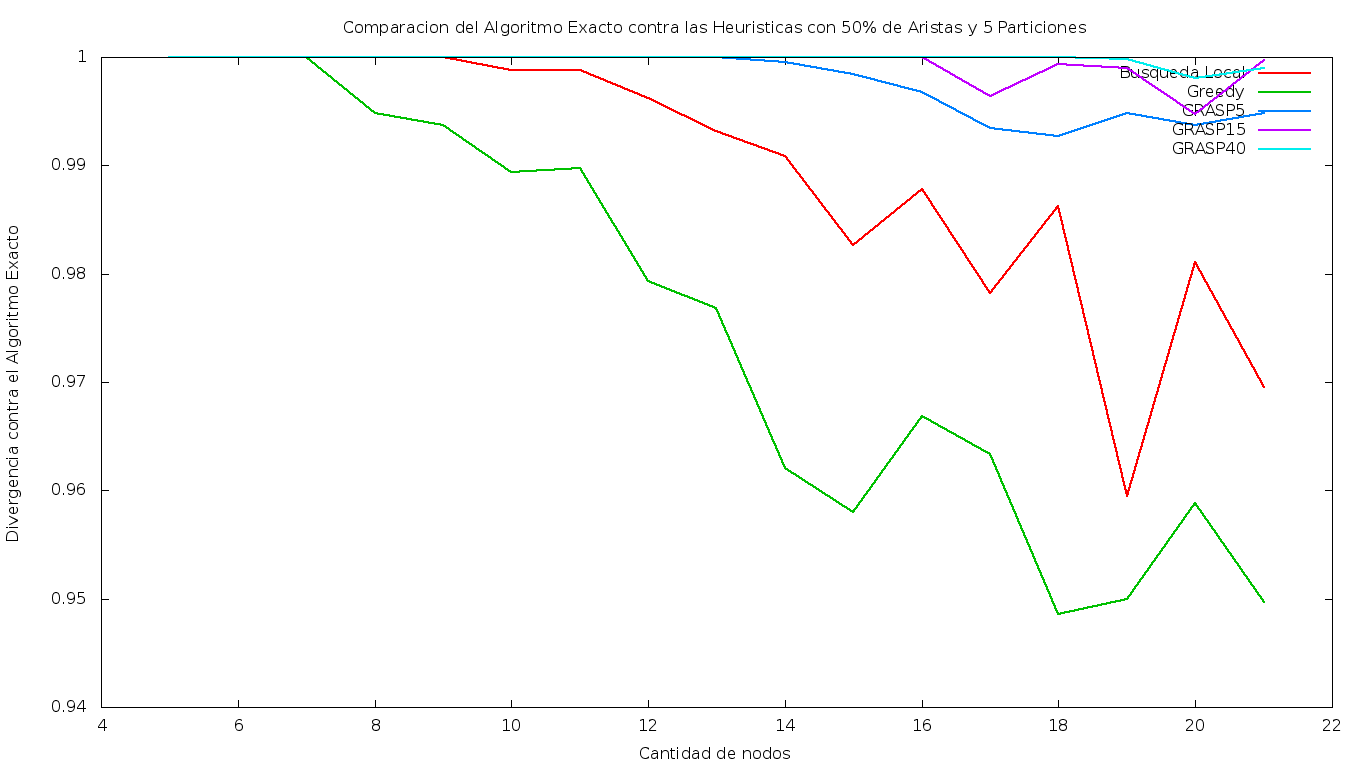
\includegraphics[scale=0.3]{finales/ComparacionesCon5Particiones50Aristas.png}
\caption{Distancias de las Heuristicas para K = 5 y 50\% de aristas}
\end{center}
\end{figure}

\begin{figure}[H]
\begin{center}
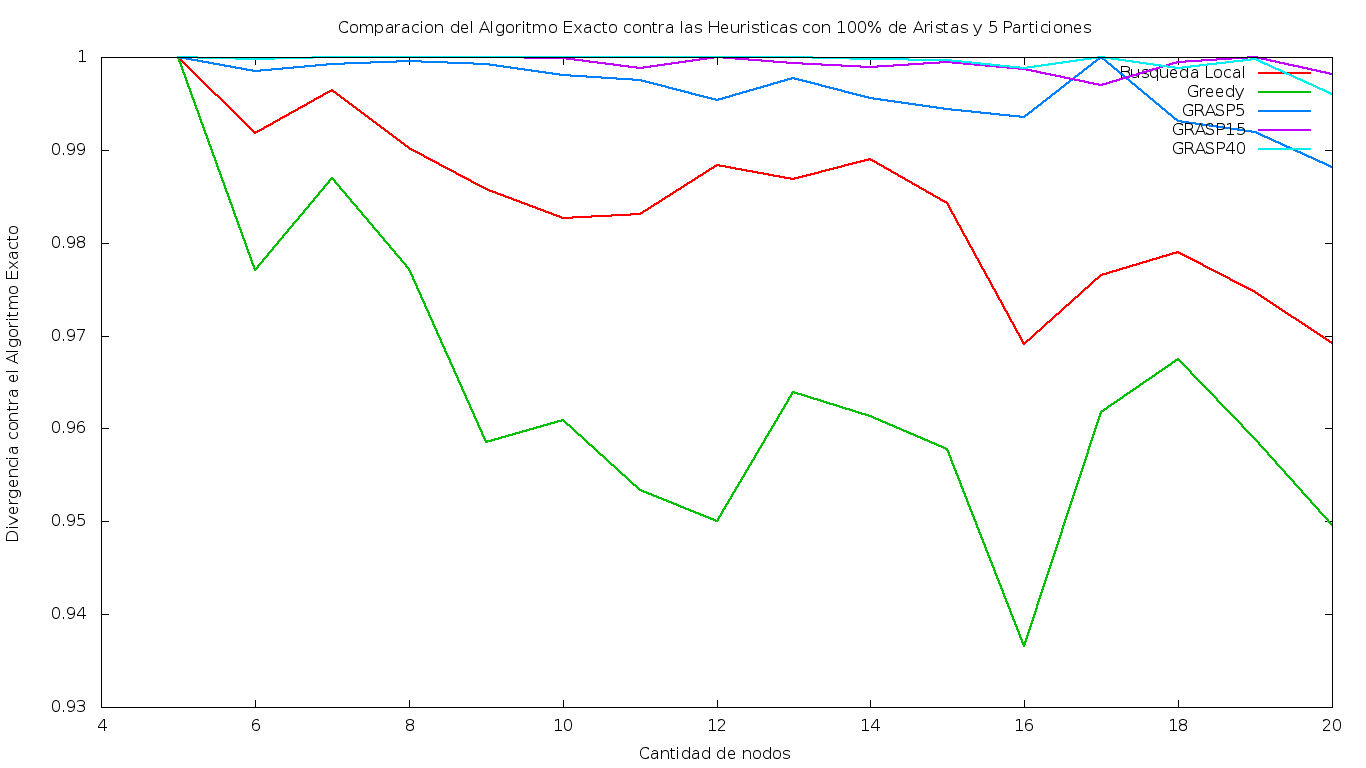
\includegraphics[scale=0.3]{finales/ComparacionesCon5Particiones100Aristas.png}
\caption{Distancias de las Heuristicas para K = 5 y 100\% de aristas}
\end{center}
\end{figure}

\subsubsection{6 Particiones}

\begin{figure}[H]
\begin{center}
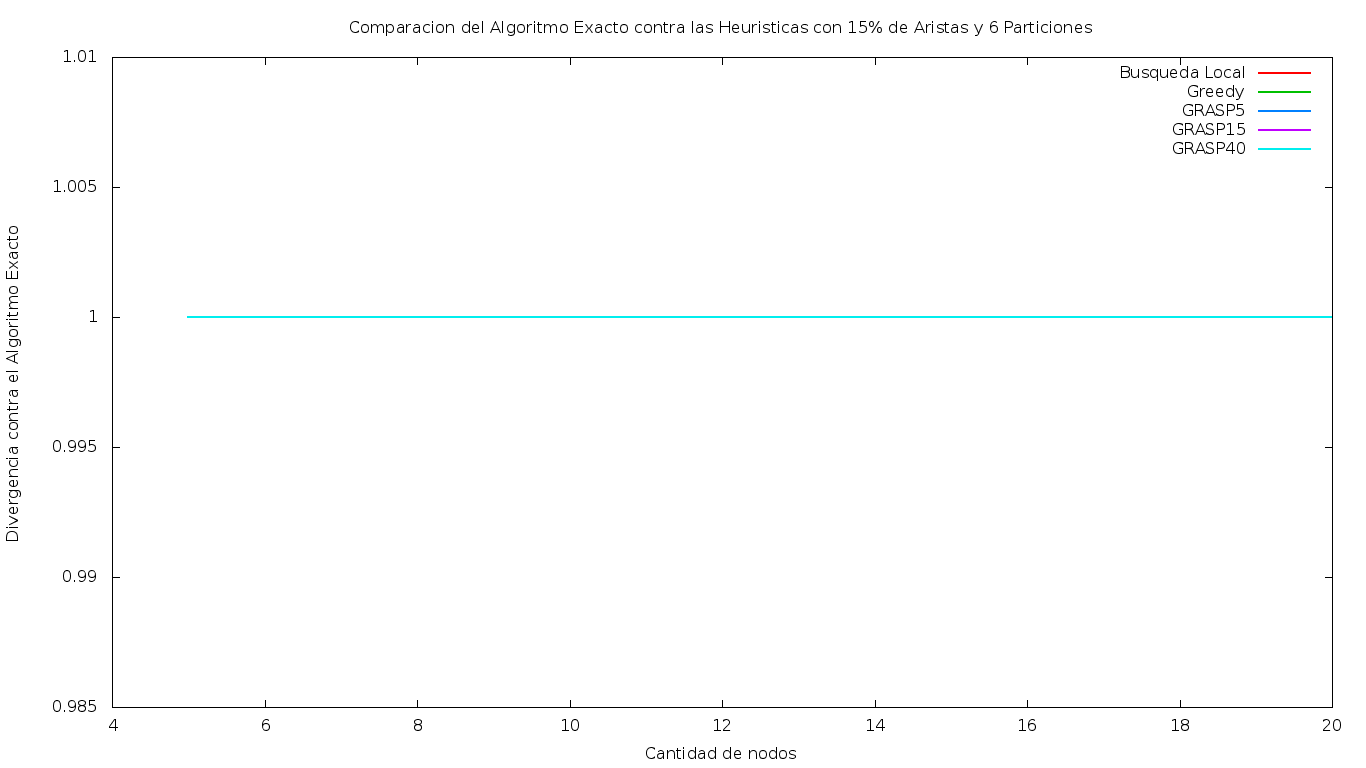
\includegraphics[scale=0.3]{finales/ComparacionesCon6Particiones15Aristas.png}
\caption{Distancias de las Heuristicas para K = 6 y 15\% de aristas}
\end{center}
\end{figure}

\begin{figure}[H]
\begin{center}
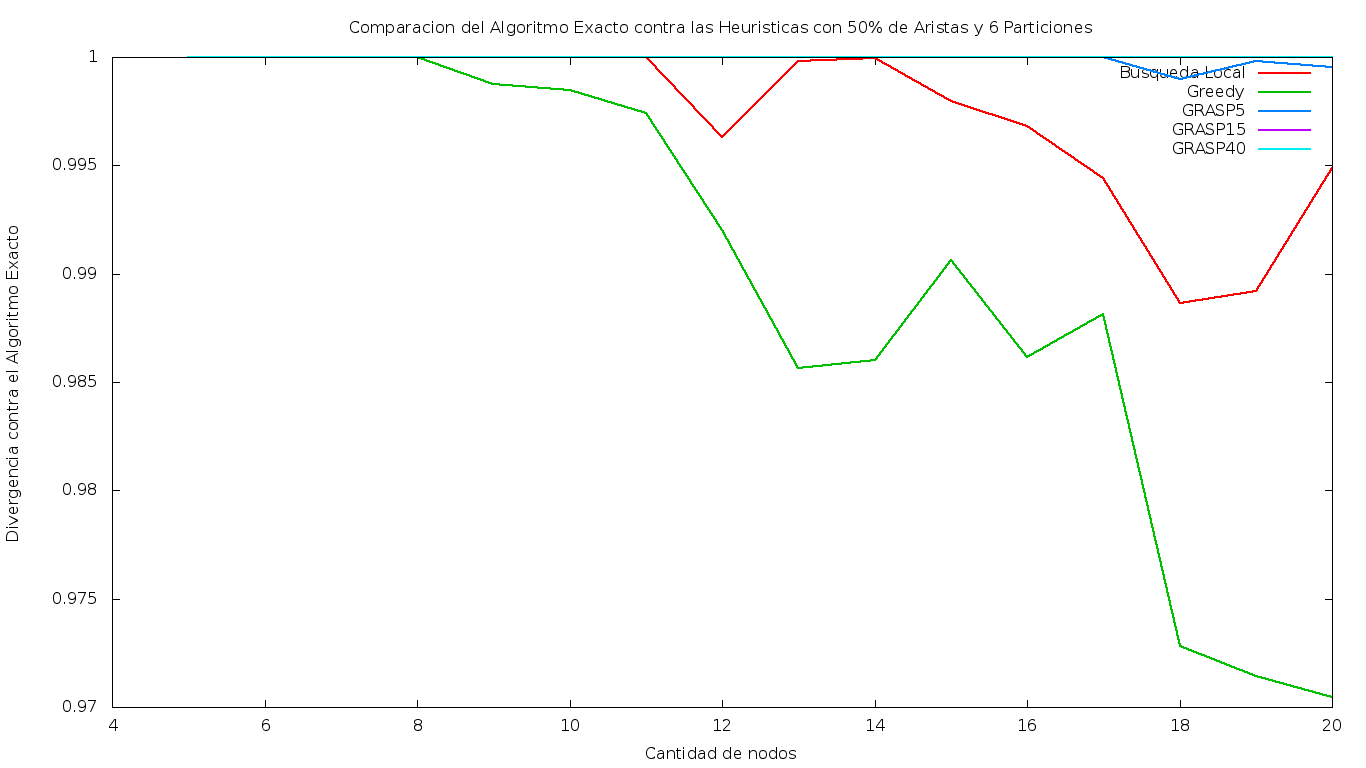
\includegraphics[scale=0.3]{finales/ComparacionesCon6Particiones50Aristas.png}
\caption{Distancias de las Heuristicas para K = 6 y 50\% de aristas}
\end{center}
\end{figure}

\begin{figure}[H]
\begin{center}
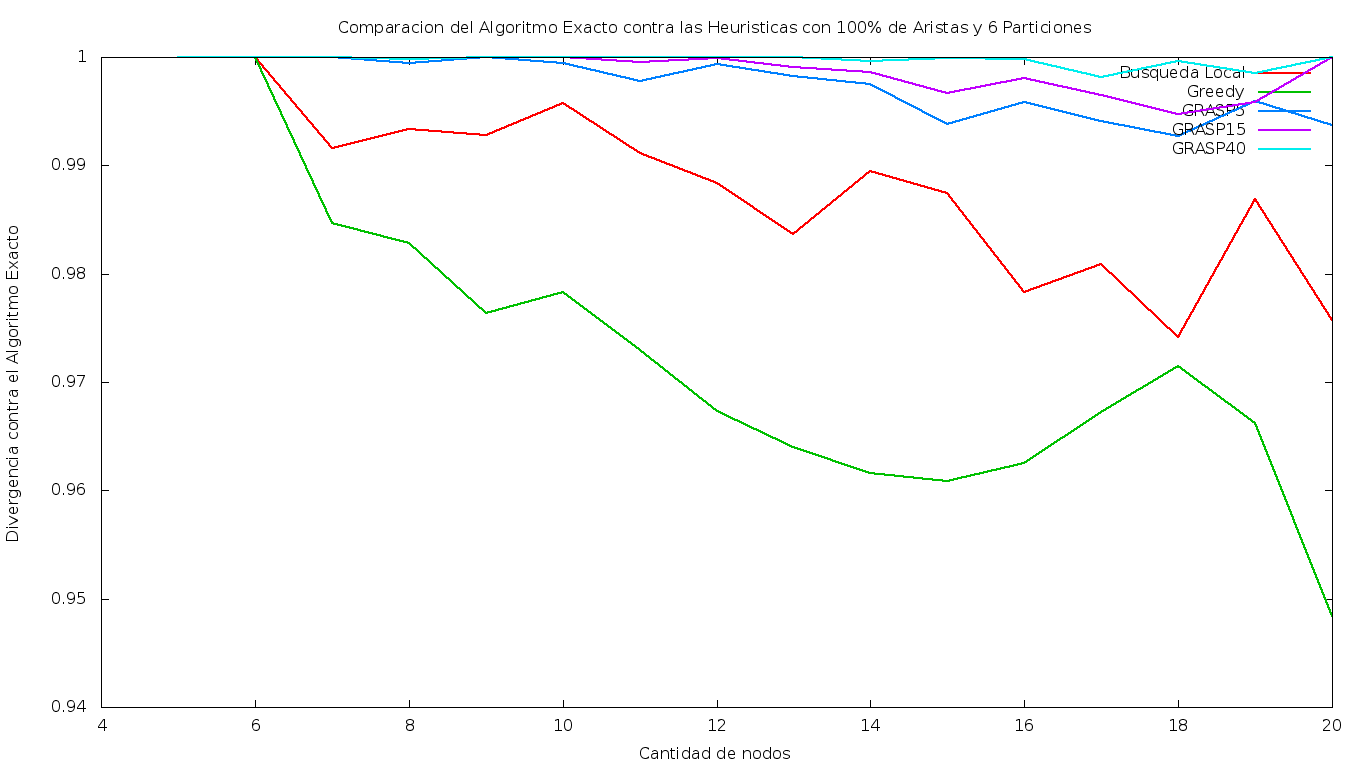
\includegraphics[scale=0.3]{finales/ComparacionesCon6Particiones100Aristas.png}
\caption{Distancias de las Heuristicas para K = 6 y 100\% de aristas}
\end{center}
\end{figure}

\subsubsection{7 Particiones}

\begin{figure}[H]
\begin{center}
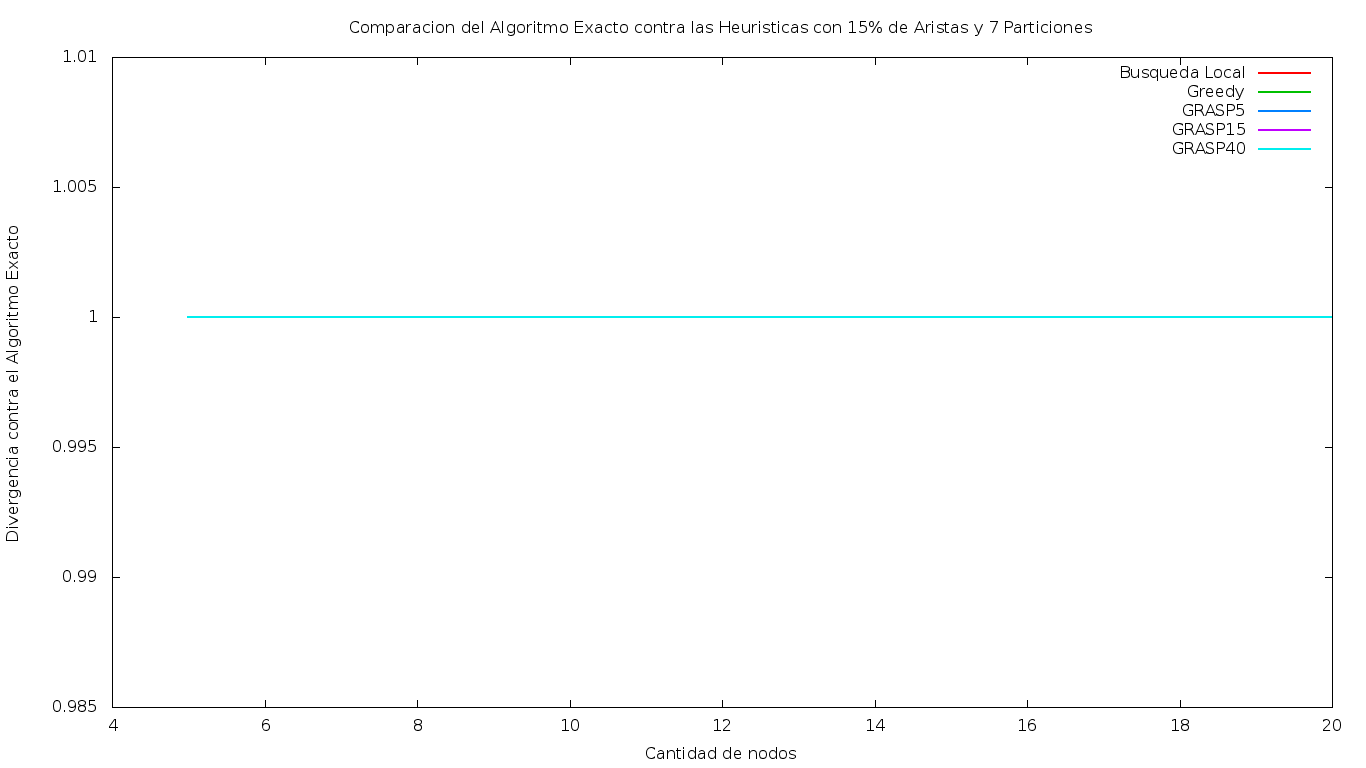
\includegraphics[scale=0.3]{finales/ComparacionesCon7Particiones15Aristas.png}
\caption{Distancias de las Heuristicas para K = 7 y 15\% de aristas}
\end{center}
\end{figure}

\begin{figure}[H]
\begin{center}
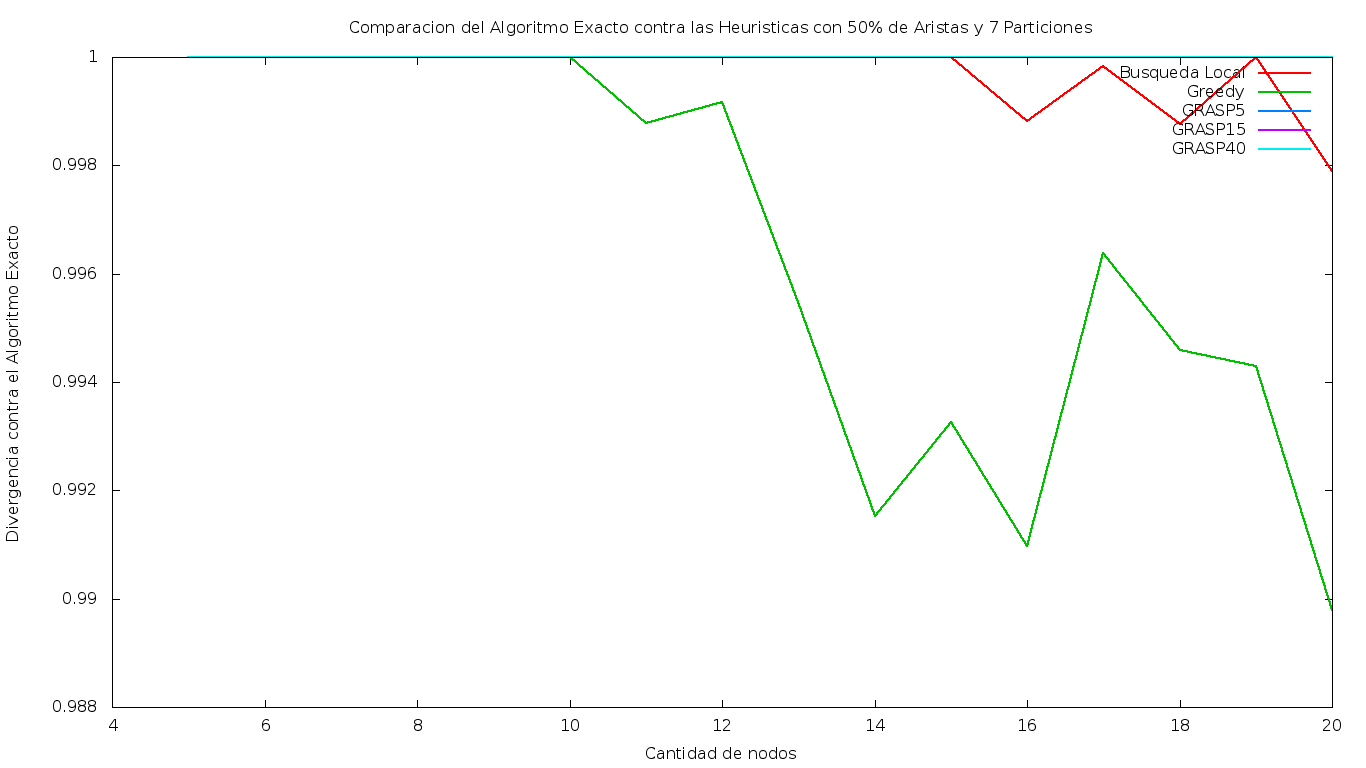
\includegraphics[scale=0.3]{finales/ComparacionesCon7Particiones50Aristas.png}
\caption{Distancias de las Heuristicas para K = 7 y 50\% de aristas}
\end{center}
\end{figure}

\begin{figure}[H]
\begin{center}
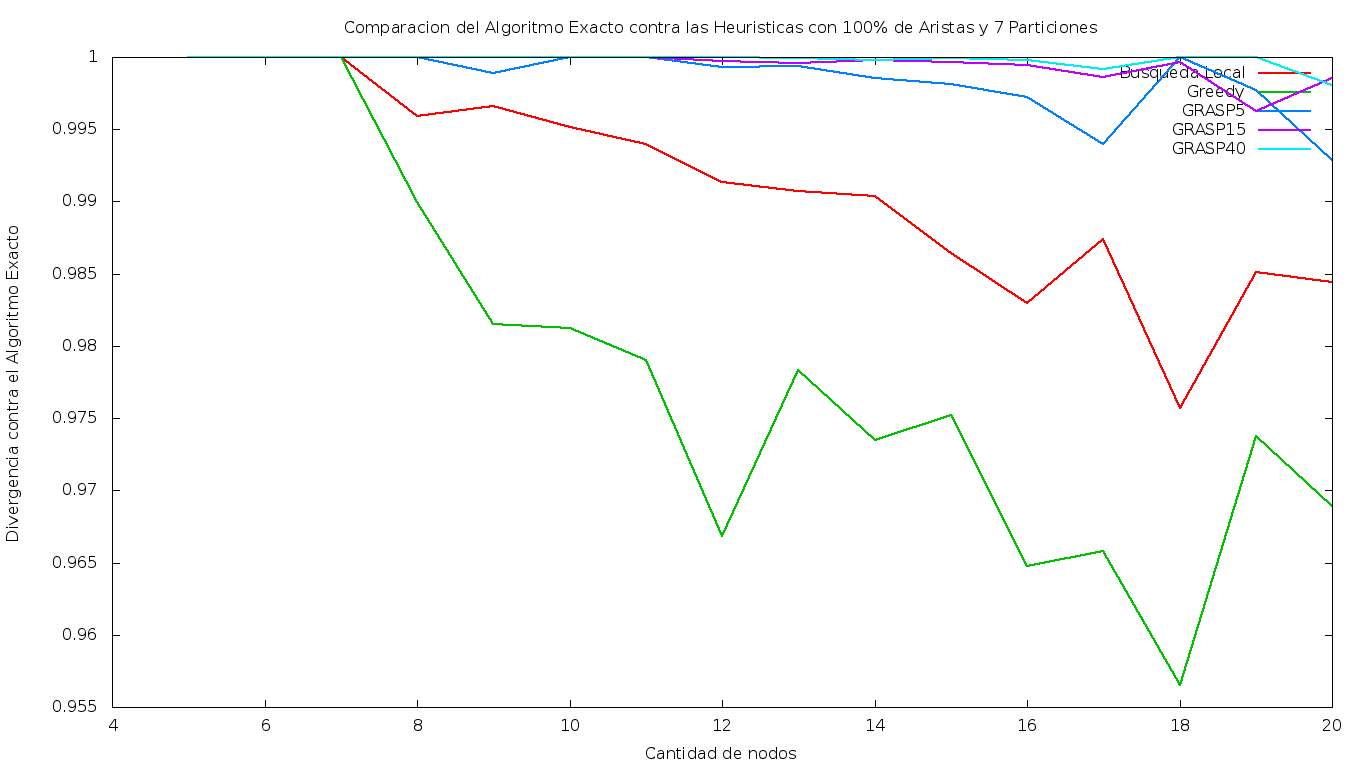
\includegraphics[scale=0.3]{finales/ComparacionesCon7Particiones100Aristas.png}
\caption{Distancias de las Heuristicas para K = 7 y 100\% de aristas}
\end{center}
\end{figure}



Podemos ver como a medida que aumenta la cantida de nodos los valores de divergencia de las Heur\'isticas comienzan a aumentar.\\

Otro punto f\'acilmente apreciable es que la Heur\'istica Greedy es la que mayor distancia tiene con respecto a la soluci\'on Exacta para todos los valores de n y cantidad de particiones, seguida por Busqueda Local y luego como, es de esperarse, los GRASP con distinta cantidad de iteraciones.\\

Volvemos a ver como al aumentar la cantidad de particiones, en funcion de las densidades del grafo, para grafos menos densos, en todos los algoritmos las soluciones se acercan mucho mas a la Ecxacta. Como ya lo mencionamos en alg\'un momento esto debe ser produco de la libertad que tengo de colocar los nodos al tener un grafo poco denso (que probablemnte tanga una gran cantidad de nodos aislados y una menor aristas intrapartici\'ones).

No podemos apreciar bien los valores de los distintos GRASP con sus respectiva cantidad de repeticiones, ya que para estas cantidades de nodos y particiones todos devuelven resultados muy similares.\\
Por este motivo vamos a realizar m\'as experimentos pero excuptuando al algoritmo exacto para poder correr instancias m\'as grandes.


\section{Divergencia para instancias mayores}

\subsubsection{5 Particiones}

\begin{figure}[H]
\begin{center}
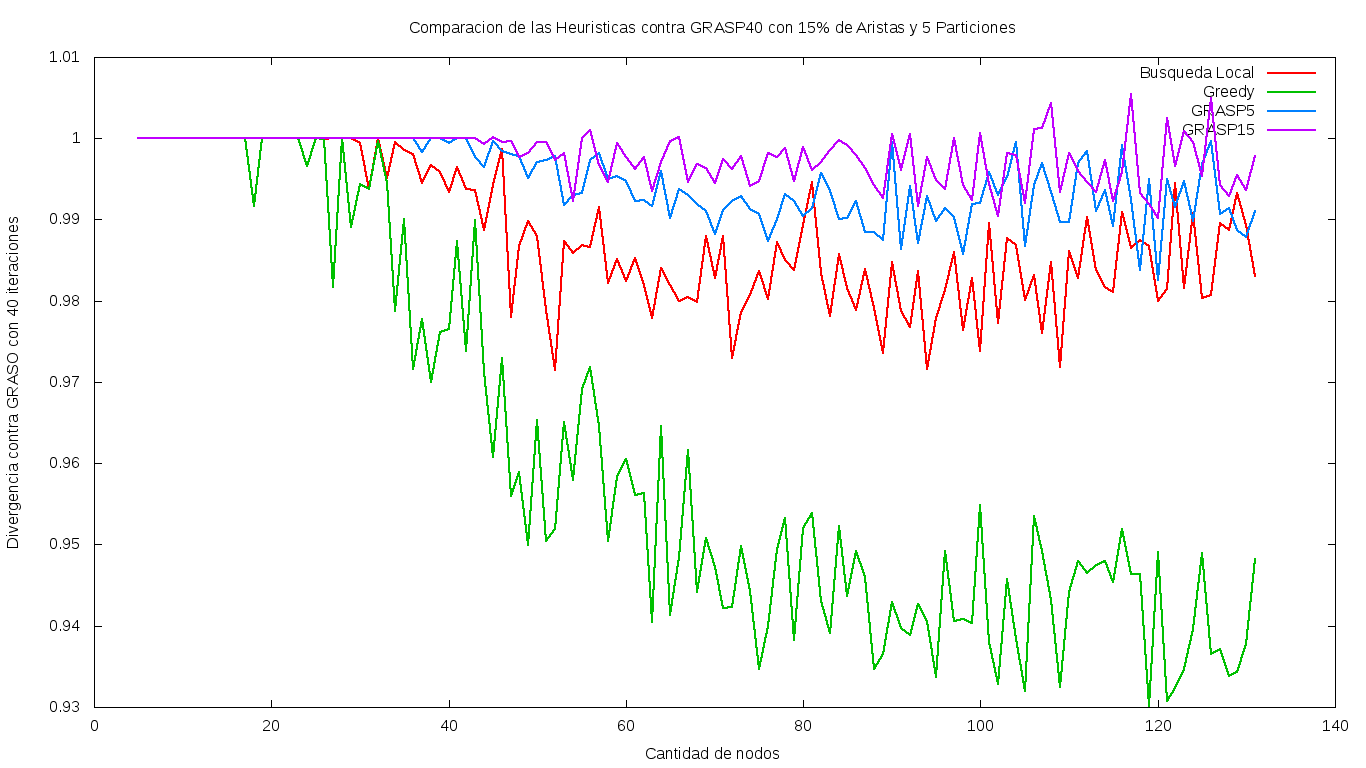
\includegraphics[scale=0.3]{finales/muchosComparacionesCon5Particiones15Aristas.png}
\caption{Distancias de las soluciones para K = 5 y 15\% de aristas}
\end{center}
\end{figure}

\begin{figure}[H]
\begin{center}
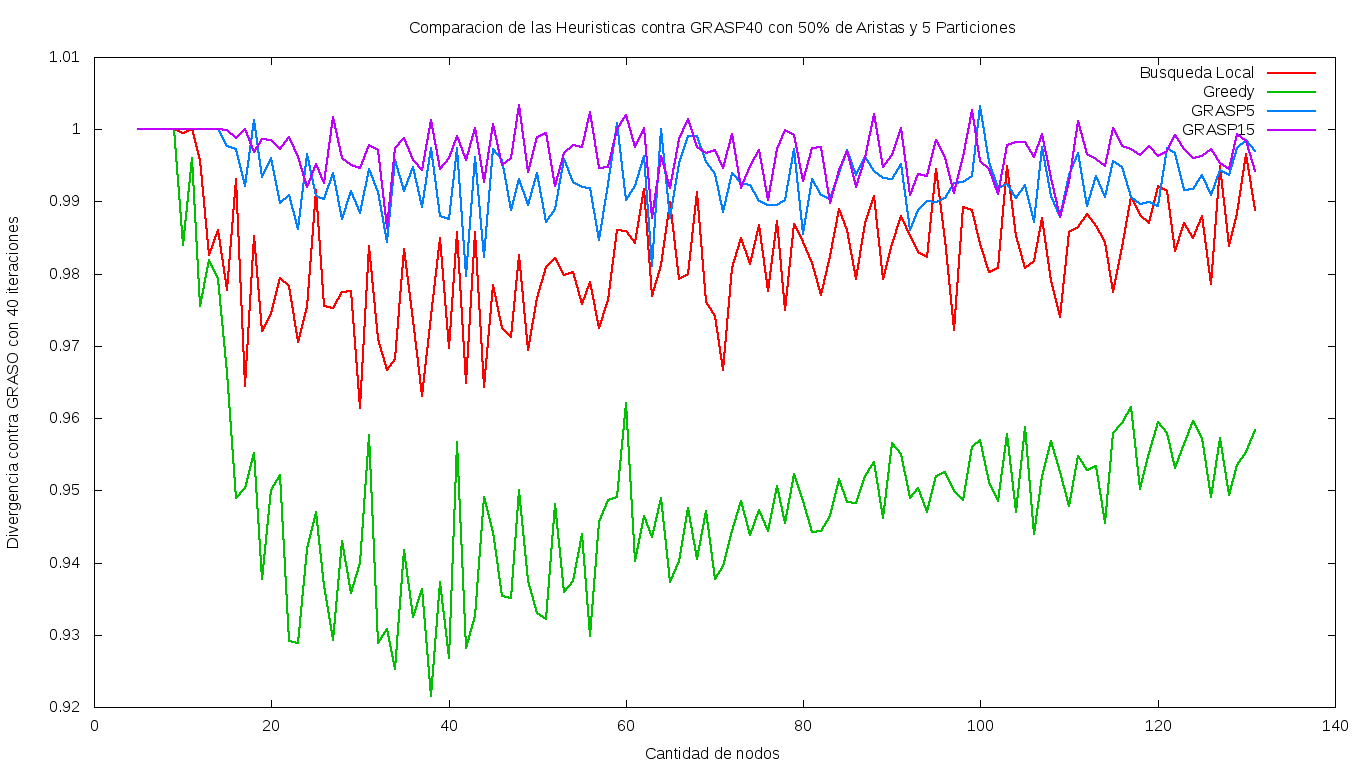
\includegraphics[scale=0.3]{finales/muchosComparacionesCon5Particiones50Aristas.png}
\caption{Distancias de las solucioens para K = 5 y 50\% de aristas}
\end{center}
\end{figure}

\begin{figure}[H]
\begin{center}
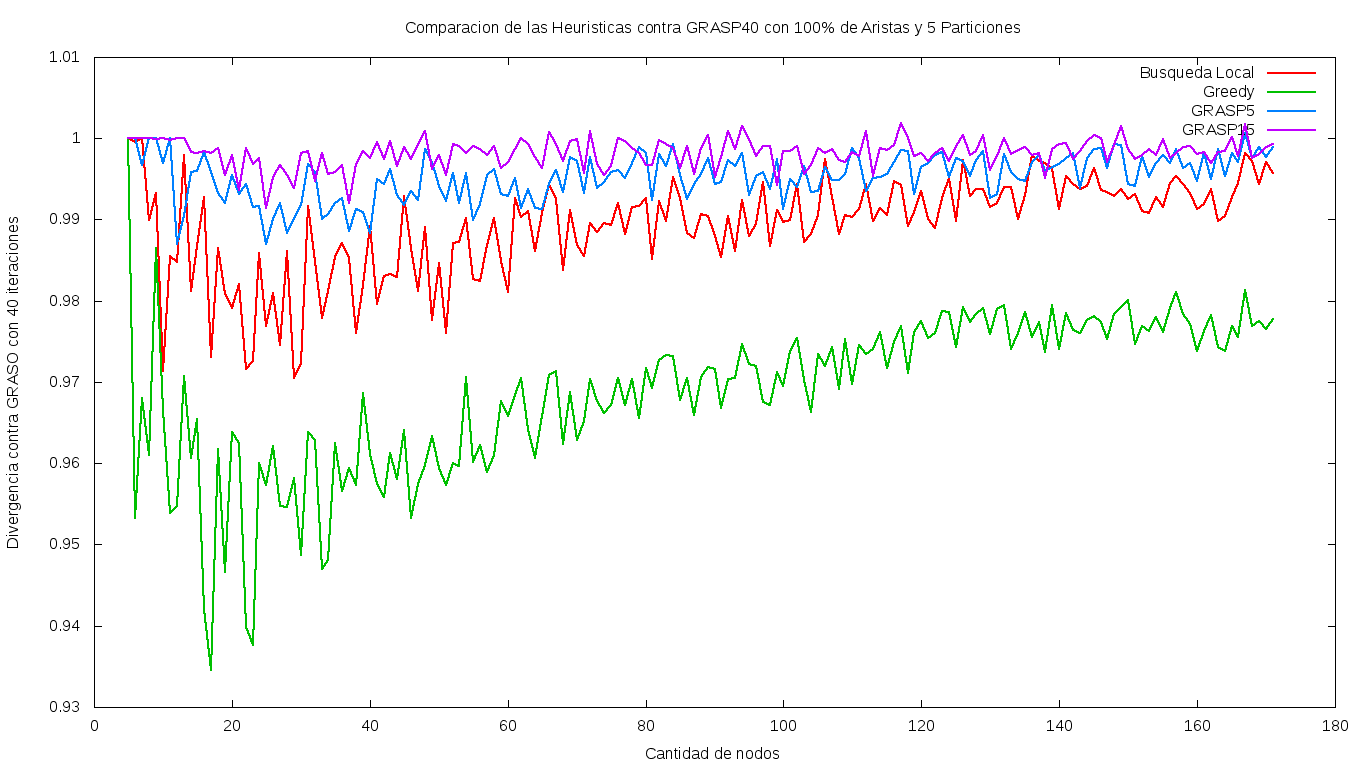
\includegraphics[scale=0.3]{finales/muchosComparacionesCon5Particiones100Aristas.png}
\caption{Distancias de las solucioens para K = 5 y 100\% de aristas}
\end{center}
\end{figure}

\subsubsection{30 Particiones}

\begin{figure}[H]
\begin{center}
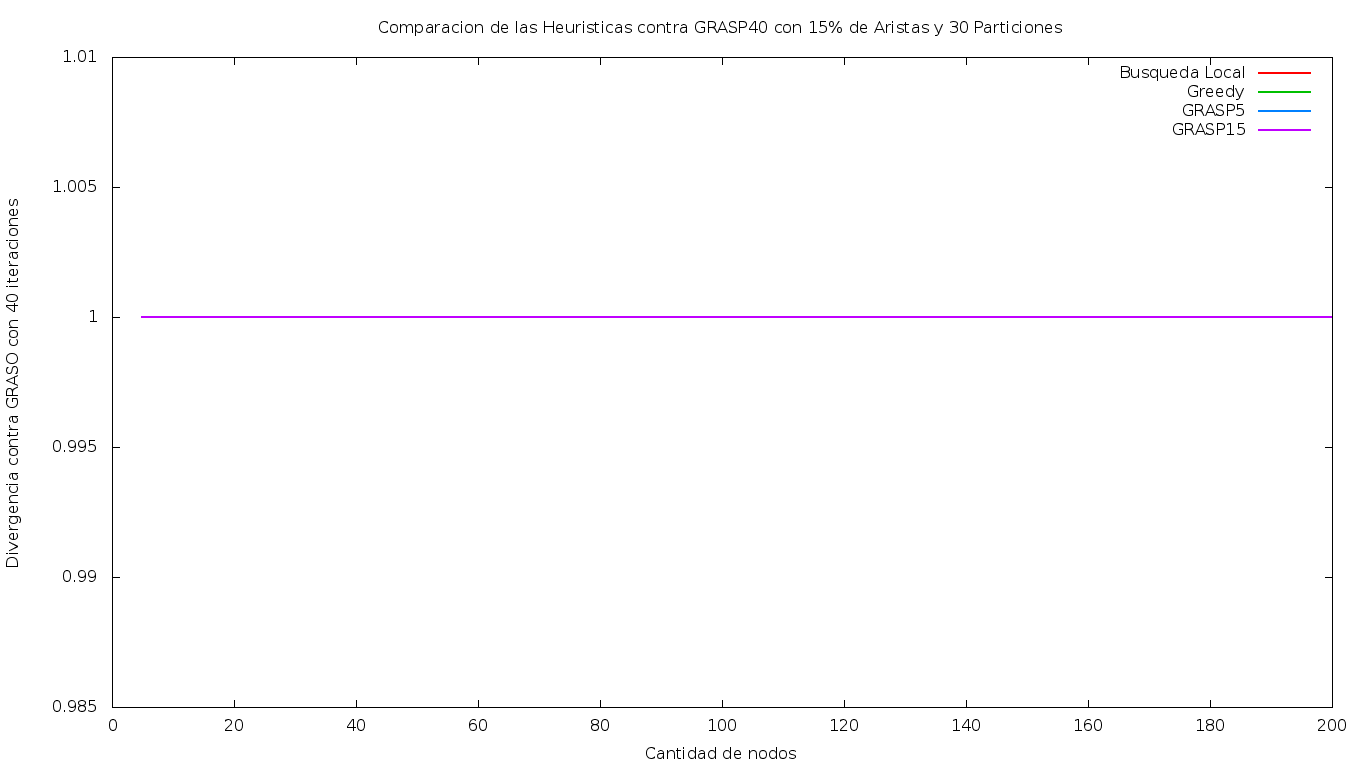
\includegraphics[scale=0.3]{finales/muchosComparacionesCon30Particiones15Aristas.png}
\caption{Distancias de las soluciones para K = 30 y 15\% de aristas}
\end{center}
\end{figure}

\begin{figure}[H]
\begin{center}
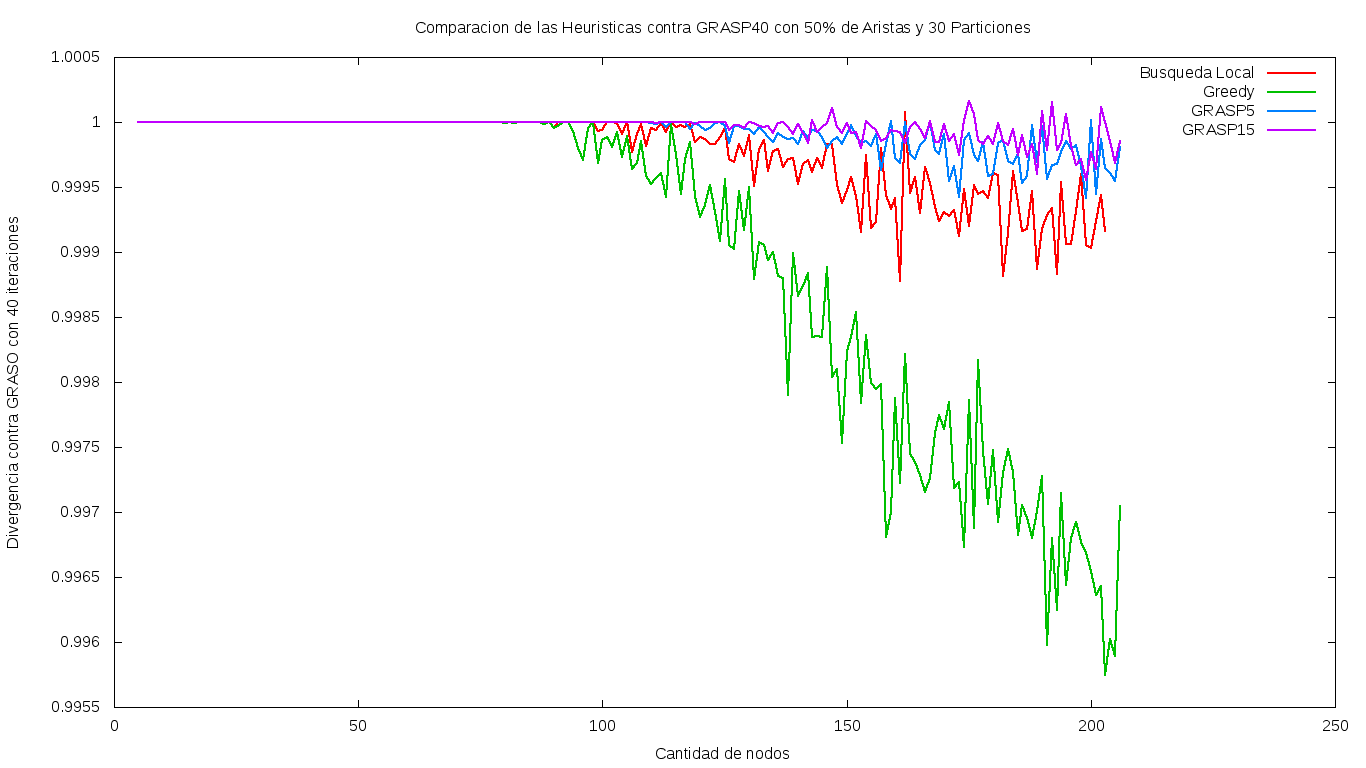
\includegraphics[scale=0.3]{finales/muchosComparacionesCon30Particiones50Aristas.png}
\caption{Distancias de las solucioens para K = 30 y 50\% de aristas}
\end{center}
\end{figure}

\begin{figure}[H]
\begin{center}
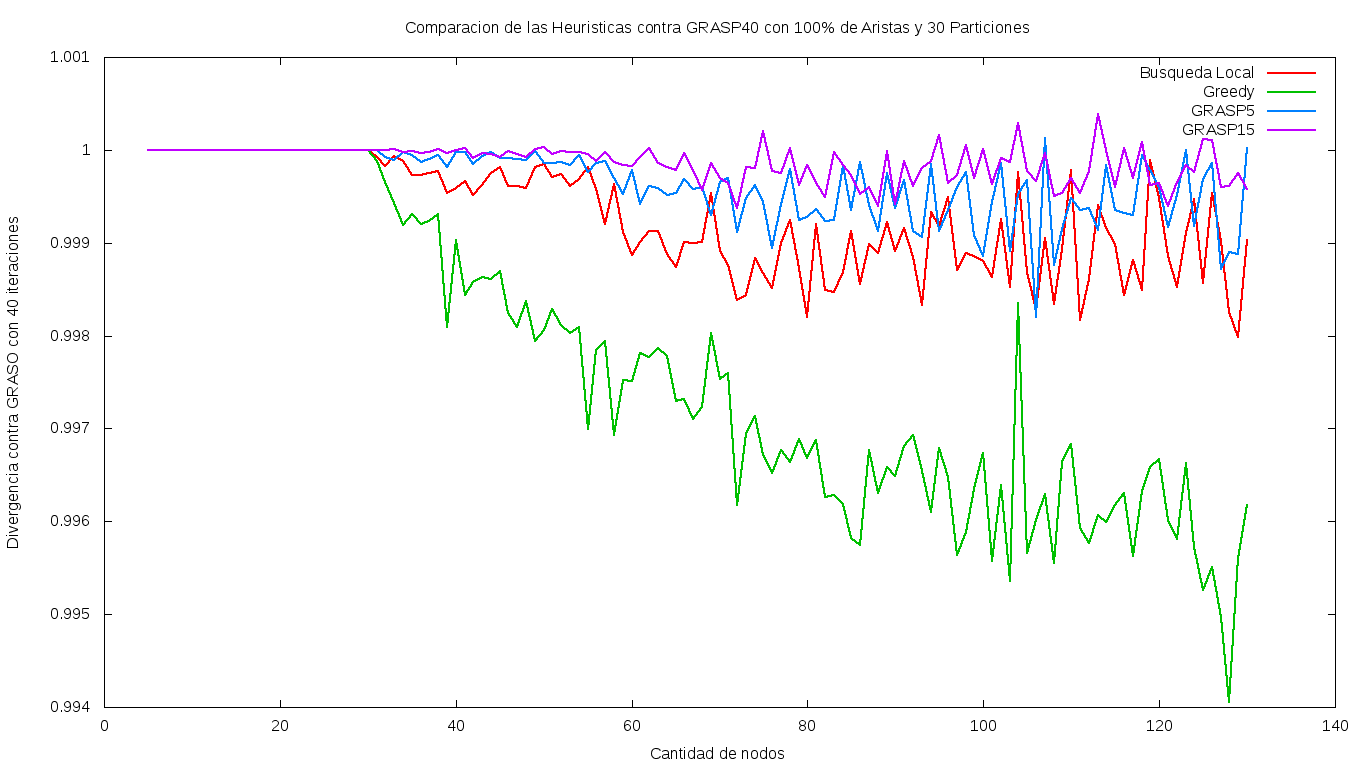
\includegraphics[scale=0.3]{finales/muchosComparacionesCon30Particiones100Aristas.png}
\caption{Distancias de las solucioens para K = 30 y 100\% de aristas}
\end{center}
\end{figure}

\subsubsection{70 Particiones}

\begin{figure}[H]
\begin{center}
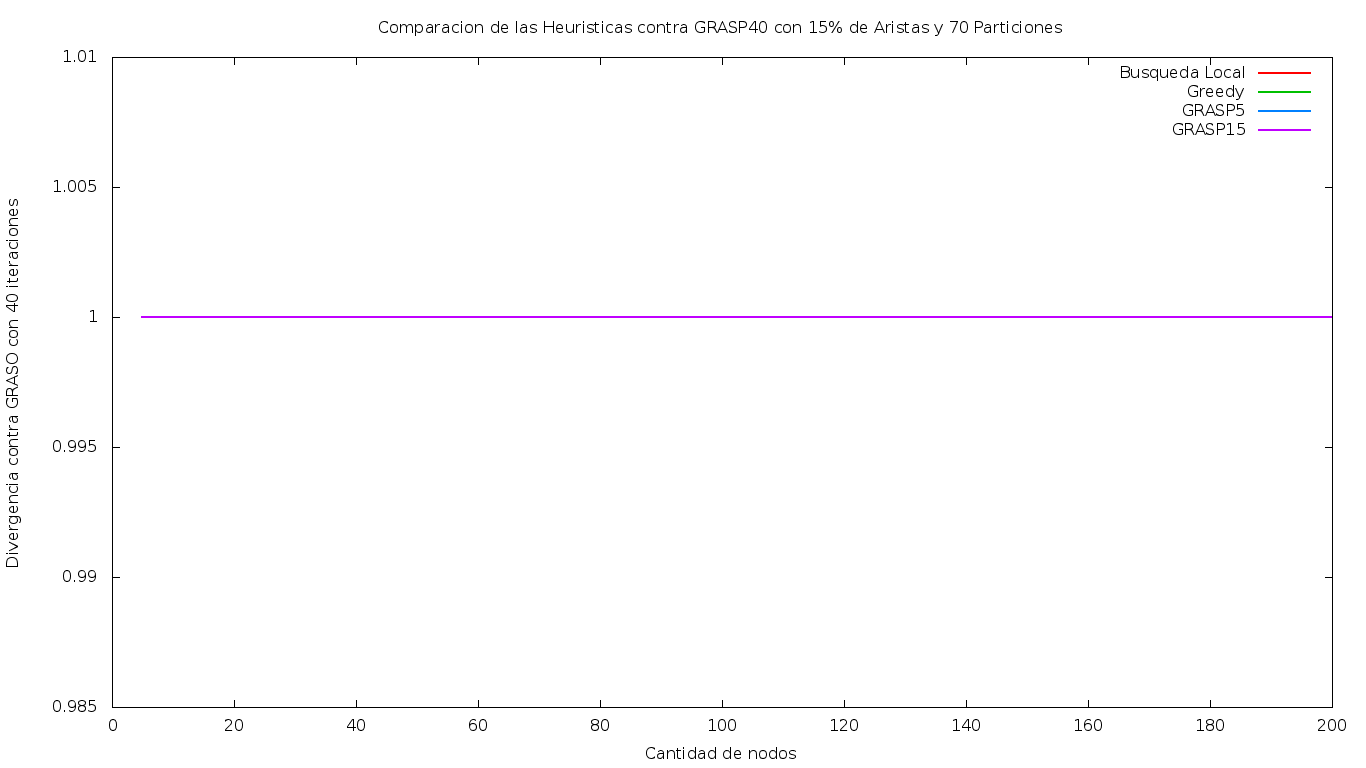
\includegraphics[scale=0.3]{finales/muchosComparacionesCon70Particiones15Aristas.png}
\caption{Distancias de las soluciones para K = 70 y 15\% de aristas}
\end{center}
\end{figure}

\begin{figure}[H]
\begin{center}
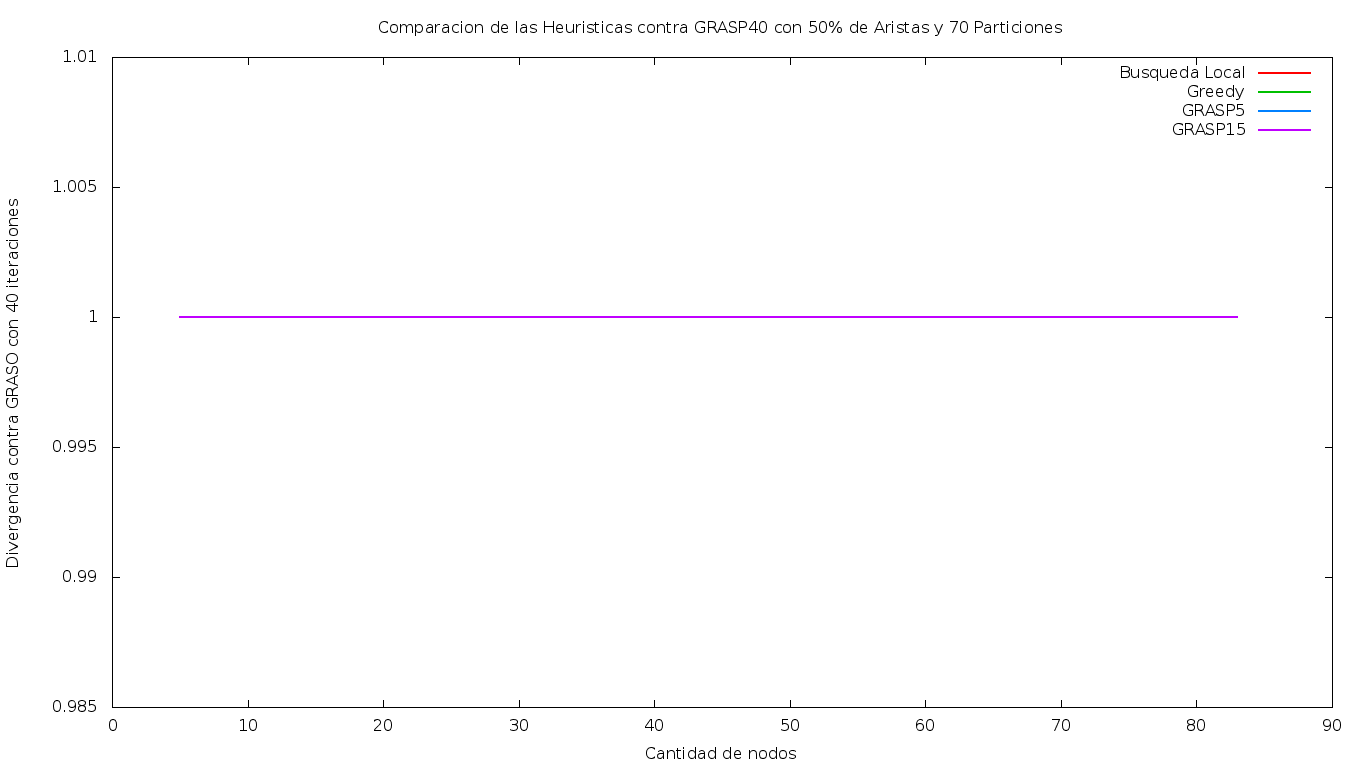
\includegraphics[scale=0.3]{finales/muchosComparacionesCon70Particiones50Aristas.png}
\caption{Distancias de las solucioens para K = 70 y 50\% de aristas}
\end{center}
\end{figure}

\begin{figure}[H]
\begin{center}
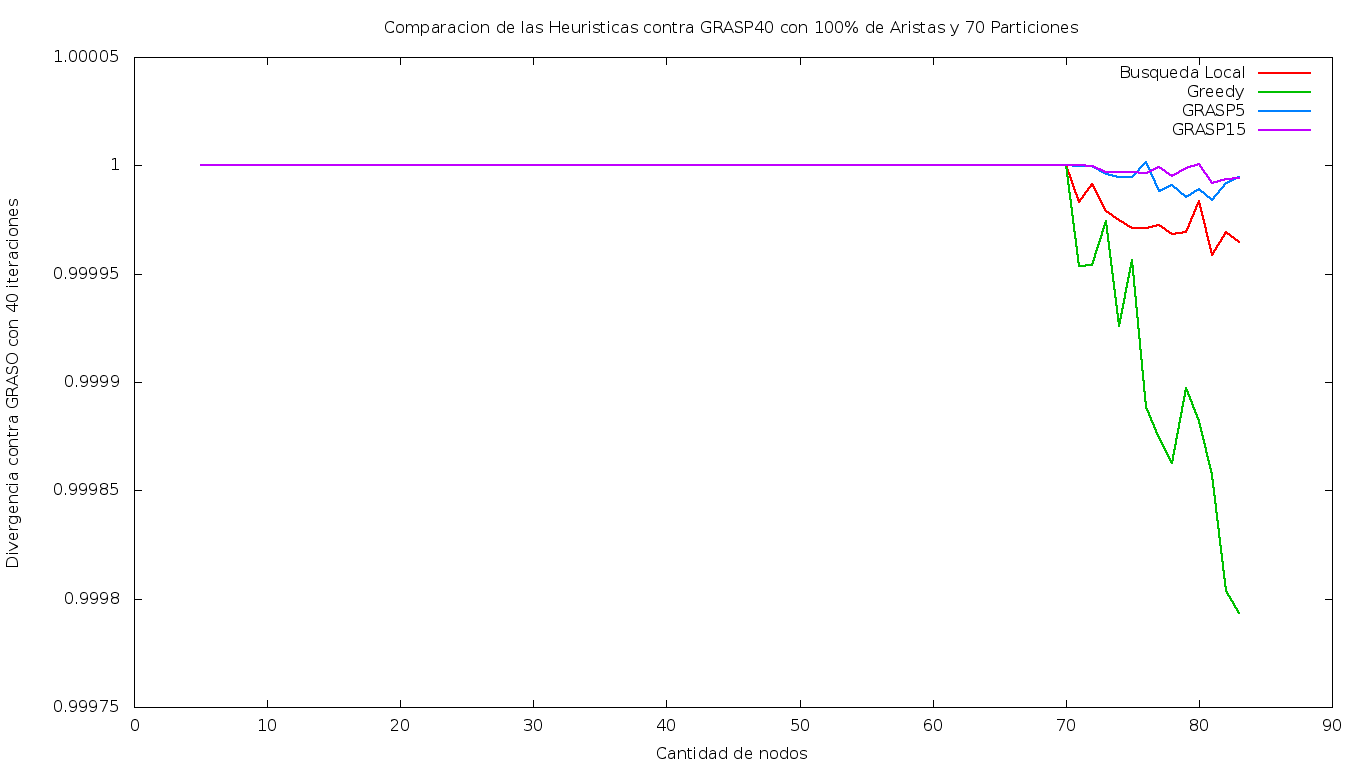
\includegraphics[scale=0.3]{finales/muchosComparacionesCon70Particiones100Aristas.png}
\caption{Distancias de las solucioens para K = 70 y 100\% de aristas}
\end{center}
\end{figure}